\section{Rendu en temps réel}

Notre objectif est d'avoir un rendu en temps réel, c'est-à-dire une fréquence minimale de 30 images par seconde. Si tout le bâtiment devait être calculé à chaque image, il est évident que nous n'aurions pas un rendu assez rapide. Comme expliqué dans le chapitre \emph{Analyse} de ce rapport, la librairie WebGL que l'on utilise (three.js) offre du \textit{Backface et Frustum culling}. Grâce à ces avantages, il est déjà plus simple d'effectuer un rendu en temps réel.

Une solution imaginée pour gagner en performance était d'effectuer une découpe du bâtiment en de nombreux morceaux (Schéma en figure \ref{fig:rendering-slice}). Chacune de ces pièces serait sauvegardée dans deux versions différentes: une en haute qualité et l'autre en moins bonne qualité. A partir de là, l'idée était de mettre en place un système \emph{LoD (Level of Detail)} \cite{wiki-lod}, ce qui signifie qu'on charge le modèle en bonne qualité seulement si la caméra est proche, sinon on charge le modèle de qualité moins bonne. Cela dit, les tests effectués n'ont pas montré de réel gain de performance. Il a été conclu que cela était dû au \textit{culling} déjà géré par three.js.

\begin{figure}
\centering
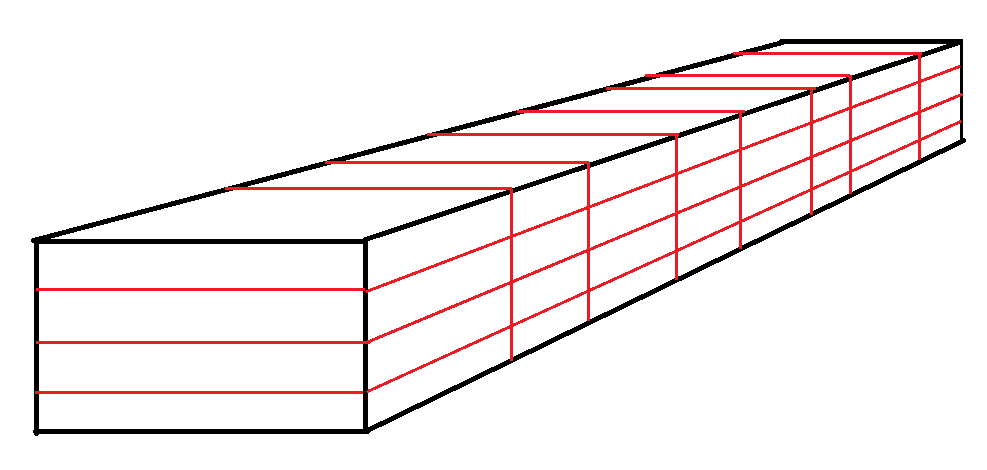
\includegraphics[width=0.7\linewidth]{rendering-Slice}
\caption{Schéma d'une découpe possible du bâtiment.}
\label{fig:rendering-slice}
\end{figure}

\subsection{Textures indexées}
Un problème de performance est apparu après avoir exporté la version texturée du modèle. Afin d'appliquer plusieurs textures sur un même objet avec \textit{Autodesk 3ds max}, il faut utiliser des \emph{Multi/Sub-Object Material}. Il s'agit, en fait, d'une liste de matériaux indexés. On l'applique à notre objet et, ensuite, on définit quel indice du matériau la face affiche. Cependant, après avoir utilisé ce genre de matériau sur le modèle, le nombre d'images par seconde sur mobile est descendu aux alentours de deux à trois. L'analyse a fait remarquer que le \textit{renderer} est appelé environ 5000 fois et, sans les textures, il n'est appelé que 30 à 40 fois. Le problème est issu du fait que, pour chaque fragment, il doit changer de texture. Et c'est précisément cette partie qui lui prend énormément de temps. La solution adoptée est de classer notre géométrie par textures, ainsi le \textit{renderer} ne doit changer de textures qu'un nombre limité de fois et, par voie de conséquence, le nombre d'images par seconde est de nouveau en dessus de 30.

\subsection{Matériel utilisé}
L'application offre au minimum 30 images par seconde. Mais ce nombre d'images par seconde n'est pas très objectif sans les informations du matériel utilisé. Les tests effectués sur un ordinateur portable ont été réalisés avec un \emph{HP EliteBook 8570w}:

\begin{description}[align=right, labelwidth=3cm]
	\item [OS] Microsoft Windows 10
	\item [Chipset]	Mobile Intel® QM77 Express Chipset
	\item [CPU] 3rd Generation Intel® CoreTM i7 Quad-Core
	\item [GPU] A NVIDIA Quadro K2000M
\end{description}

Pour les tests sur smartphone, c'est un \emph{Motorola Nexus 6} qui a été utilisé:

\begin{description}[align=right, labelwidth=3cm]
	\item [OS] 	Android OS v6.0 (Marshmallow)
	\item [Chipset]	Qualcomm Snapdragon 805
	\item [CPU] Quad-core 2.7 GHz Krait 450
	\item [GPU] Adreno 420
\end{description}
